%!TEX root = Programmierparadigmen.tex
\chapter{Prolog}
\index{Prolog|(}

Prolog ist eine Programmiersprache, die das logische Programmierparadigma
befolgt.

Eine interaktive Prolog-Sitzung startet man mit \texttt{swipl}.

In Prolog definiert man Terme.
\section{Erste Schritte}
\subsection{Hello World}
Speichere folgenden Quelltext als \texttt{hello-world.pl}:
\inputminted[linenos, numbersep=5pt, tabsize=4, frame=lines, label=hello-world.hs]{prolog}{scripts/prolog/hello-world.pl}

Kompiliere ihn mit \texttt{gplc hello-world.pl}. Es wird eine
ausführbare Datei erzeugt.

\section{Syntax}
In Prolog gibt es Prädikate, die Werte haben. Prädikate werden immer klein geschrieben.
So kann das Prädikat \texttt{farbe} mit den Werten \texttt{rot}, \texttt{gruen},
\texttt{blau}, \texttt{gelb} - welche auch immer klein geschrieben werden - wie
folgt definiert werden:

\inputminted[numbersep=5pt, tabsize=4]{prolog}{scripts/prolog/praedikat-farbe.pl}

\begin{itemize}
    \item Terme werden durch \texttt{,} mit einem logischem \textbf{und} verknüpft.
    \item Ungleichheit wird durch \texttt{\=} ausgedrückt.
\end{itemize}

So ist folgendes Prädikat \texttt{nachbar(X, Y)} genau dann wahr, wenn $X$
und $Y$ Farben sind und $X \neq Y$ gilt:

\inputminted[numbersep=5pt, tabsize=4]{prolog}{scripts/prolog/simple-term.pl}

\subsection{Kommentare}\xindex{Kommentare (Prolog)}
Prolog kennt zwei Kommentar-Typen:

\begin{itemize}
    \item Zeilen-Kommentare, die mit \verb+%+ beginnen
    \item Block-Kommentare, diem durch \verb+/* ... */+ markiert werden.
\end{itemize}

\subsection{= und ==}\xindex{= (Prolog)}\xindex{== (Prolog)}
In Prolog entspricht \texttt{=} dem Prädikat \texttt{=/2}. Das Prädikat \texttt{<a> = <b>} wird
erfüllt, wenn die beiden Terme \texttt{<a>} und \texttt{<b>} unifiziert werden
können.

Das Prädikat \texttt{<a> == <b>} ist im Gegensatz dazu jedoch nur erfüllt, wenn
die beiden Terme bereits identisch sind.

\begin{beispiel}[= und ==]
    \inputminted[numbersep=5pt, tabsize=4]{prolog}{scripts/prolog/equal.pl}
\end{beispiel}

Weitere Informationen: \url{http://stackoverflow.com/a/8220315/562769}

\subsection{! (Cut)}\xindex{"! (Cut, Prolog)}%
Das \texttt{!} wird in Prolog als \textit{cut} bezeichnet. Ein Cut verhindert
Backtracking nach dem cut.

Die Klauseln eines Prädikates werden von Prolog von links nach rechts evaluiert.
Prolog bindet einen Wert an eine Variable in der linkesten Klausel. Wenn diese
Klausel als \texttt{true} ausgewertet wird, dann versucht Prolog die nächste
Klausel auszuwerten. Falls nicht, wird eine neuer Wert an die momentan
betrachtete Klausel gebunden.

Da Klauseln über logische UND verbunden sind, führt eine nicht erfüllbare
Klausel dazu, dass das gesamte Prädikat als \texttt{false} evaluiert wird.

Der cut ist ein Gate: Sind die Klauseln vor dem cut ein mal wahr, werden die
Werte festgelegt.

\subsection{Arithmetik}
Die Auswertung artihmetischer Ausdrücke muss in Prolog explizit durch \texttt{is}
durchgeführt werden:

\inputminted[numbersep=5pt, tabsize=4]{prolog}{scripts/prolog/arithmetik.pl}

Dabei müssen alle Variablen, die im Term rechts von \texttt{is} vorkommen,
istanziiert sein:

\inputminted[numbersep=5pt, tabsize=4]{prolog}{scripts/prolog/arithmetik-fail.pl}

Arithmetische Ausdrücke können mit \texttt{=:= , =\textbackslash= , < , <= , > , >=}
verglichen werden.

\begin{beispiel}[Arithmetik in Prolog\footnotemark]
    \begin{bspenum}
        \item \inputminted[numbersep=5pt, tabsize=4]{prolog}{scripts/prolog/even.pl}\xindex{even (Prolog)@\texttt{even} (Prolog)}
        \item \inputminted[numbersep=5pt, tabsize=4]{prolog}{scripts/prolog/fibonacci2.pl}\xindex{Prolog!Fibonacci}
    \end{bspenum}
\end{beispiel}
\footnotetext{WS 2013 / 2014, Folie 237f}

\subsection{Listen}
Das Atom \texttt{[]} ist die leere Liste.

Mit der Syntax \texttt{[K|R]} wird eine Liste in den Listekopf \texttt{K} und
den Rest der Liste \texttt{R} gesplitet:

\inputminted[numbersep=5pt, tabsize=4]{prolog}{scripts/prolog/liste-basic.pl}

Einen Test \texttt{member(X, Liste)}, der \texttt{True} zurückgibt wenn \texttt{X}
in \texttt{Liste} vorkommt, realisiert man wie folgt:

\inputminted[numbersep=5pt, tabsize=4]{prolog}{scripts/prolog/liste-member.pl}\xindex{member}

Eine Regel \texttt{append(A, B, C)}, die die Listen \texttt{A} und \texttt{B}
zusammenfügt und als Liste \texttt{C} speichert, kann
wie folgt erstellt werden:

\inputminted[numbersep=5pt, tabsize=4]{prolog}{scripts/prolog/liste-append.pl}

Die erste Regel besagt, dass das Hinzufügen der leeren Liste zu einer Liste
\texttt{L} immer noch die Liste \texttt{L} ist.

Die zweite Regel besagt: Wenn die Liste \texttt{R} und \texttt{L} die Liste \texttt{T}
ergeben, dann ergibt die Liste, deren Kopf \texttt{X} ist und deren Rumpf \texttt{R}
ist zusammen mit der Liste \texttt{L} die Liste mit dem Kopf \texttt{X} und dem
Rumpf \texttt{T}.

\xindex{split}Übergibt man \texttt{append(X,Y,[1,2,3,4,5])}, so werden durch Reerfüllung alle
Möglichkeiten durchgegangen, wie man die Liste \texttt{[1,2,3,4,5]} splitten kann.

Die Länge einer Liste \texttt{L} kann durch folgendes Prädikat ermittelt werden:\xindex{length(?List, ?Int)@\texttt{length(?List, ?Int)}}%

\inputminted[numbersep=5pt, tabsize=4]{prolog}{scripts/prolog/list-length.pl}

\underline{Hinweis}: Da es das Prädikat \texttt{length(?List, ?Int)} bereits gibt,
musste dieses Prädikat \texttt{lengthof} genannt werden.

Weitere nützliche Standard-Listenprädikate sind:\xindex{sort(+List, -Sorted)@\texttt{sort(+List, -Sorted)}}
\inputminted[numbersep=5pt, tabsize=4]{prolog}{scripts/prolog/standard-list-predicates.pl}

\underline{Hinweis}: \texttt{sort} entfernt Duplikate, \texttt{msort} hingegen nicht.

Eine Liste kann mit \texttt{rev/2}\xindex{rev/2@\texttt{rev/2}} umgedreht werden:
\inputminted[numbersep=5pt, tabsize=4]{prolog}{scripts/prolog/reverse-list.pl}

\subsection{Bäume}
Bäume können in Prolog wie folgt erstellt werden:

\inputminted[numbersep=5pt, tabsize=4]{prolog}{scripts/prolog/binary-tree-example.pl}

\begin{figure}[htp]
    \centering
     \tikzstyle{vertex}=[draw,fill=black!15,circle,minimum size=20pt,inner sep=0pt]
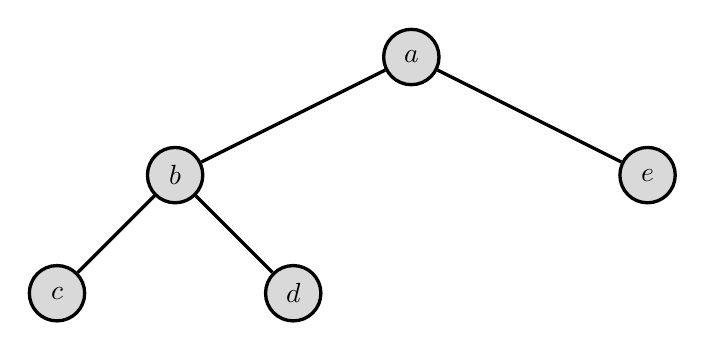
\begin{tikzpicture}[very thick,level/.style={sibling distance=60mm/#1}]
\node [vertex] (r){$a$}
  child {
    node [vertex] (a) {$b$}
    child {
      node [vertex] {$c$}
    }
    child {
      node [vertex] {$d$}
    }
  }
  child {
    node [vertex] {$e$}
  };
\end{tikzpicture}

    \caption{Binärbaum \texttt{T2}}
    \label{fig:binary-tree-t2}
\end{figure}

Dabei ist
\begin{itemize}
    \item \texttt{T0} der einzelne Knoten \texttt{a},
    \item \texttt{T1} der Baum, der \texttt{a} als Wurzel und \texttt{b} und
          \texttt{c} als Kinder hat,
    \item \texttt{T2} ist in \cref{fig:binary-tree-t2} dargestellt und
    \item \texttt{T3} ist der leere Baum.
\end{itemize}

Die folgenden Prädikate stammen von \url{https://sites.google.com/site/prologsite/prolog-problems/4}:

\subsection{Binärbaum-Check}
Das folgende Prädikate \texttt{istree/1} überprüft, ob es sich bei dem Parameter
um einen Binärbaum handelt:

\inputminted[numbersep=5pt, tabsize=4]{prolog}{scripts/prolog/istree.pl}

\subsection{Balancierte Binärbaumkonstruktion}
Das folgende Prädikate \texttt{cbal\_tree(n, T)} erstellt einen balancierten
Binärbaum mit \texttt{n} Knoten in \texttt{T}:

\inputminted[numbersep=5pt, tabsize=4]{prolog}{scripts/prolog/balancedtreeconstruction.pl}

\section{Beispiele}
\subsection{Humans}
Erstelle folgende Datei:
\inputminted[linenos, numbersep=5pt, tabsize=4, frame=lines, label=human.pro]{prolog}{scripts/prolog/human.pro}

Kompiliere diese mit
\inputminted[numbersep=5pt, tabsize=4]{bash}{scripts/prolog/human.sh}

Dabei wird eine \texttt{a.out} Datei erzeugt, die man wie folgt
nutzen kann:
\inputminted[numbersep=5pt, tabsize=4]{bash}{scripts/prolog/human-2.sh}

\subsection{Splits}
\inputminted[linenos, numbersep=5pt, tabsize=4, frame=lines, label=splits.pl]{prolog}{scripts/prolog/splits.pl}

Dieses skript soll man \texttt{swipl -f test.pl} aufrufen. Dann erhält man:

\inputminted[numbersep=5pt, tabsize=4]{prolog}{scripts/prolog/splits.sh}

\subsection{Delete}\xindex{remove}\xindex{delete}%
\inputminted[numbersep=5pt, tabsize=4]{prolog}{scripts/prolog/delete.pl}

% \subsection{Zebrarätsel}
% Folgendes Rätsel wurde von \url{https://de.wikipedia.org/w/index.php?title=Zebrar%C3%A4tsel&oldid=126585006}
% entnommen:

% \begin{enumerate}
%     \item Es gibt fünf Häuser.
%     \item Der Engländer wohnt im roten Haus.
%     \item Der Spanier hat einen Hund.
%     \item Kaffee wird im grünen Haus getrunken.
%     \item Der Ukrainer trinkt Tee.
%     \item Das grüne Haus ist direkt rechts vom weißen Haus.
%     \item Der Raucher von Altem-Gold-Zigaretten hält Schnecken als Haustiere.
%     \item Die Zigaretten der Marke Kools werden im gelben Haus geraucht.
%     \item Milch wird im mittleren Haus getrunken.
%     \item Der Norweger wohnt im ersten Haus.
%     \item Der Mann, der Chesterfields raucht, wohnt neben dem Mann mit dem Fuchs.
%     \item Die Marke Kools wird geraucht im Haus neben dem Haus mit dem Pferd.
%     \item Der Lucky-Strike-Raucher trinkt am liebsten Orangensaft.
%     \item Der Japaner raucht Zigaretten der Marke Parliaments.
%     \item Der Norweger wohnt neben dem blauen Haus.
% \end{enumerate}

% Wer trinkt Wasser? Wem gehört das Zebra?

% \inputminted[linenos, numbersep=5pt, tabsize=4, frame=lines, label=zebraraetsel.pro]{prolog}{scripts/prolog/zebraraetsel.pro}

% TODO: Zebrarätzel hinzufügen

\subsection{Zahlen generieren}
Folgendes Skript generiert durch reerfüllung die Zahlen $1, \dots, 10$:

\inputminted[numbersep=5pt, tabsize=4]{prolog}{scripts/prolog/zahlen-bis-10.pl}

\subsection{Reguläre ausdrücke}
Folgendes Beispiel stammt aus der Programmierparadigmenklausur vom WS 2013/2014
bei Prof. Dr. Snelting:

\inputminted[numbersep=5pt, tabsize=4]{prolog}{scripts/prolog/regex.pl}

\subsection{Coffeetime 01: Two Bases}

\inputminted[numbersep=5pt, tabsize=4]{prolog}{scripts/prolog/01-two-bases.prolog}

\section{Weitere Informationen}
\begin{itemize}
    \item \href{http://wiki.ubuntuusers.de/Prolog}{\path{wiki.ubuntuusers.de/Prolog}}: Hinweise zur Installation von Prolog unter Ubuntu
    \item \url{http://www.swi-prolog.org/}
\end{itemize}
\index{Prolog|)}
